\section{Correlation Structure}
\subsection{Business Series}
% \begin{lstlisting}[language=R]
% layout(1:2)
% acf(y1, main="Business Series")
% \end{lstlisting}
\vspace{-0.4cm}
\begin{figure}[H]
    \centering
    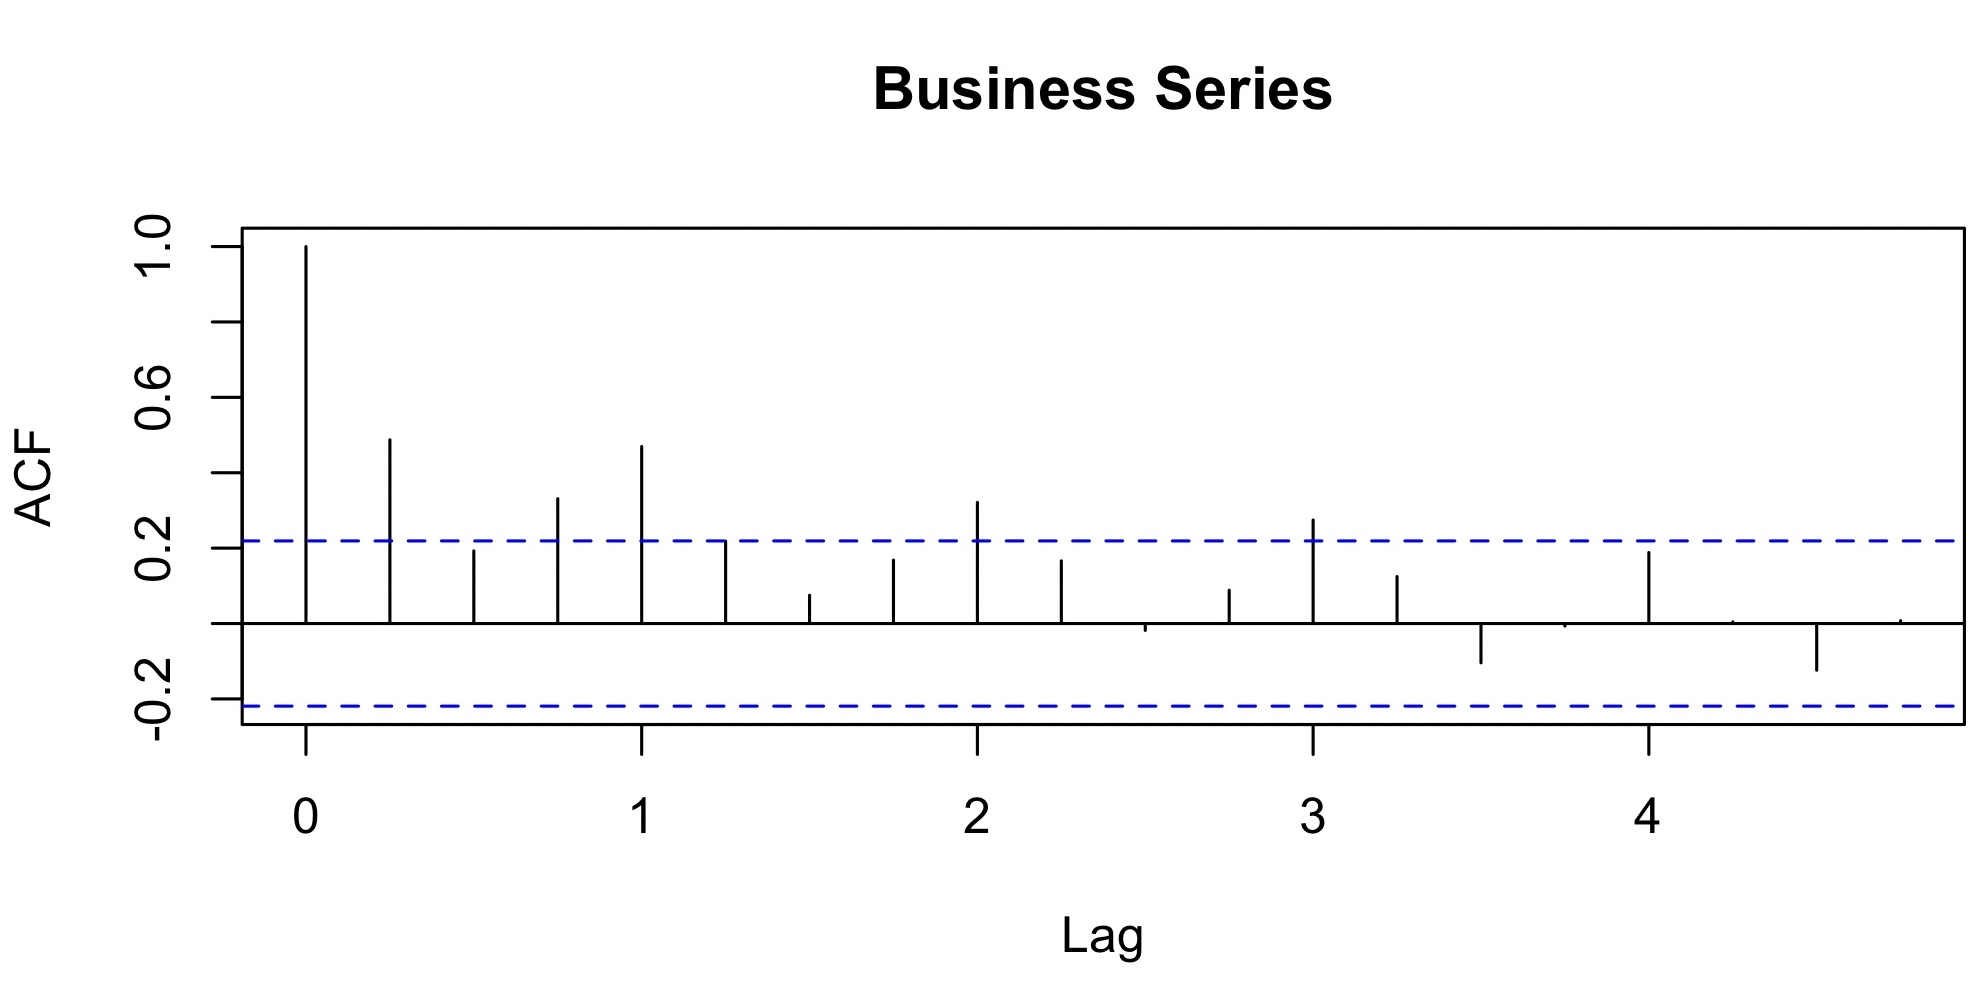
\includegraphics[width=0.65\linewidth]{fig/y1acf.jpg}
\end{figure}
\vspace{-0.4cm}
\noindent The correlogram does not decay to zero within a few lags, suggesting that the business series is unlikely to be stationary. The autocorrelations rise and fall in a repeating pattern, with peaks at lags 4, 8 and 12, reflecting a strong positive autocorrelation between pairs of quarters separated by multiples of four. That is, the same quarter in different years. This suggests a seasonal variation in the series. The autocorrelation at lag 1 is also large and positive, exceeding the dashed 95\% reference lines, so that business trips in one quarter are also correlated with trips in the following quarter. The physical interpretation is that a business quarter with above-average trips tends to be followed by a further above-average quarter. This suggests that the number of business trips in a given quarter tends to resemble that of the corresponding quarter in the following year. This behaviour is typical of a series with unremoved seasonal variation.
\vspace{0.4cm}
% \begin{lstlisting}[language=R]
% pacf(y1, main="Business Series")
% \end{lstlisting}
\begin{figure}[H]
    \centering
    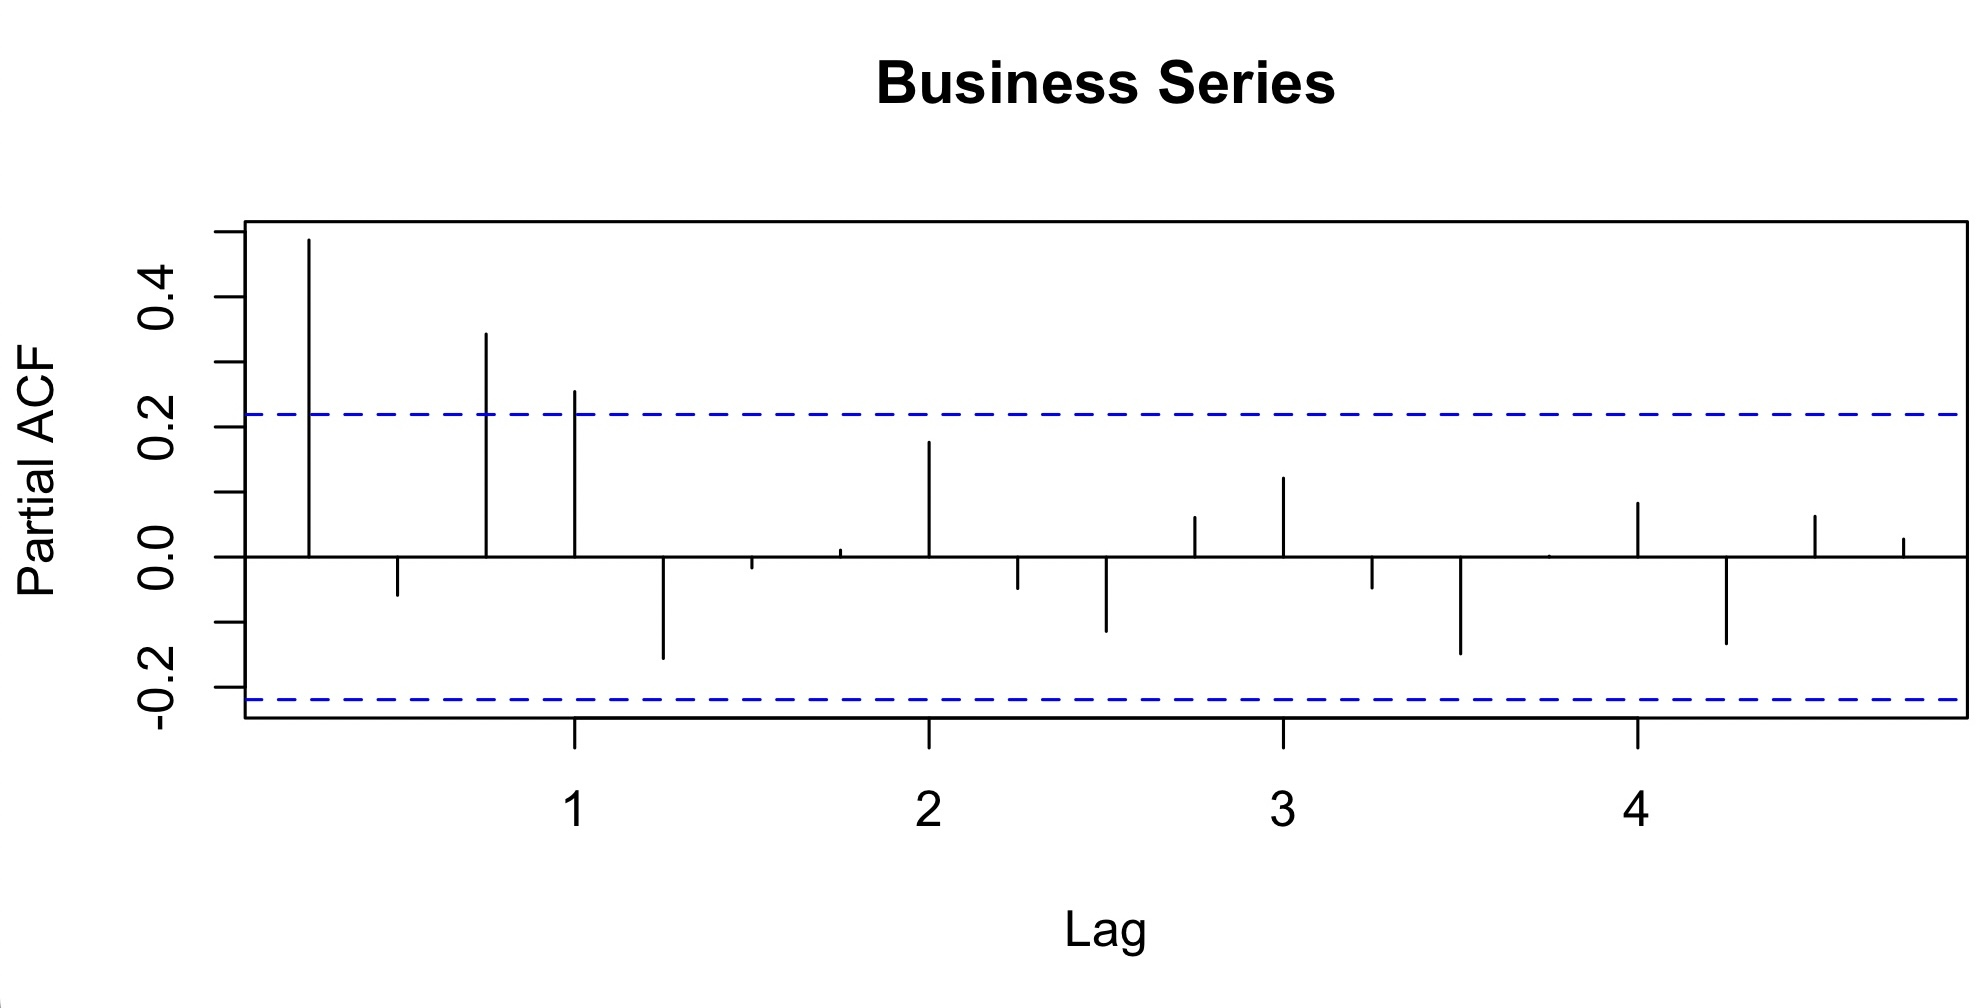
\includegraphics[width=0.65\linewidth]{fig/y1pacf.jpg}
\end{figure}

\noindent The partial autocorrelation at lag 1 is large, similar in size to the lag 1 autocorrelation, as is always the case at lag 1. Beyond lag 1, most of the partial autocorrelations lie within the reference lines, but there are significant spikes too at lag 3 and 4. Persisting correlation at a lag close to the seasonal period, once the effect of shorter lags has been removed, is again typical of a series with a seasonal component still present. \\

\noindent Taken together, the acf and pacf indicate that the business series is \textbf{non-stationary}, and that trend and seasonal effects would need to be identified and removed before the random component could reasonably be treated as stationary.

\subsection{Holiday Series}

\vspace{-0.4cm}
\begin{figure}[H]
    \centering
    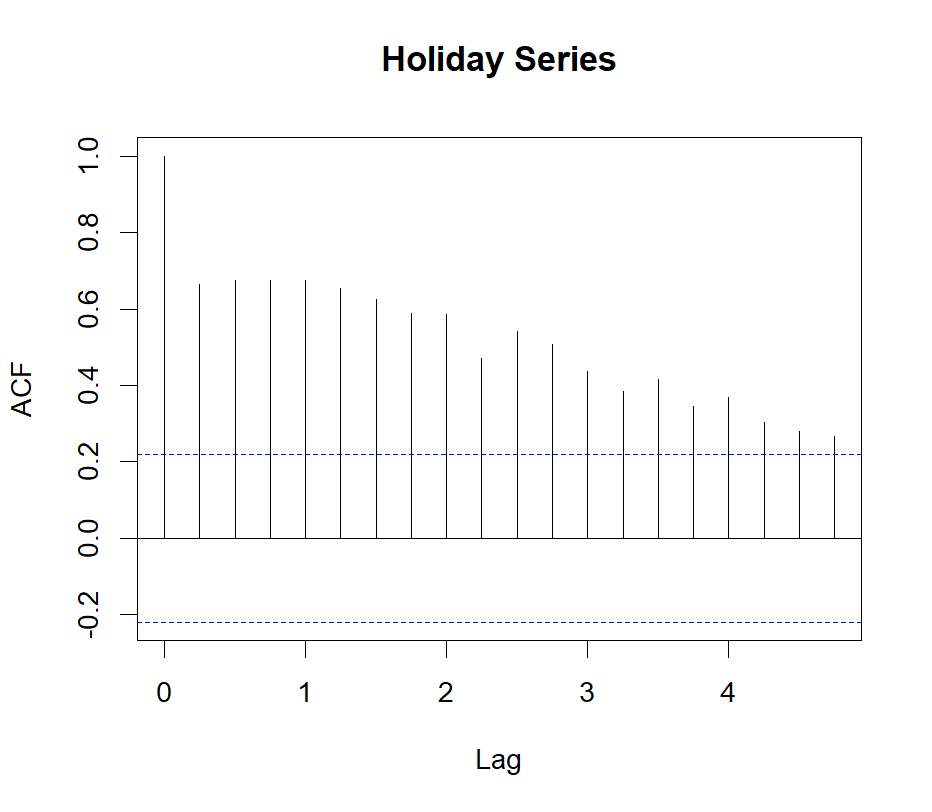
\includegraphics[width=0.65\linewidth]{fig/y2acf.png}
\end{figure}
\vspace{-0.4cm}

\noindent \noindent The ACF does not decay to zero quickly and remains significantly positive over many lags, indicating strong autocorrelation and persistence in the series. The gradual decline of the autocorrelations suggests that the series is unlikely to be stationary. This behaviour is consistent with the upward trend observed in the time plot, where the number of holiday trips increases over time.

\noindent The ACF does not show strong repeating spikes at seasonal lags, suggesting that the seasonal pattern is not dominant in the autocorrelation structure of the original series. Instead, the high autocorrelation across consecutive lags indicates that observations close together in time tend to have similar values. This suggests that the series contains a strong trend component rather than purely random fluctuations.



\vspace{0.4cm}

\begin{figure}[H]
    \centering
    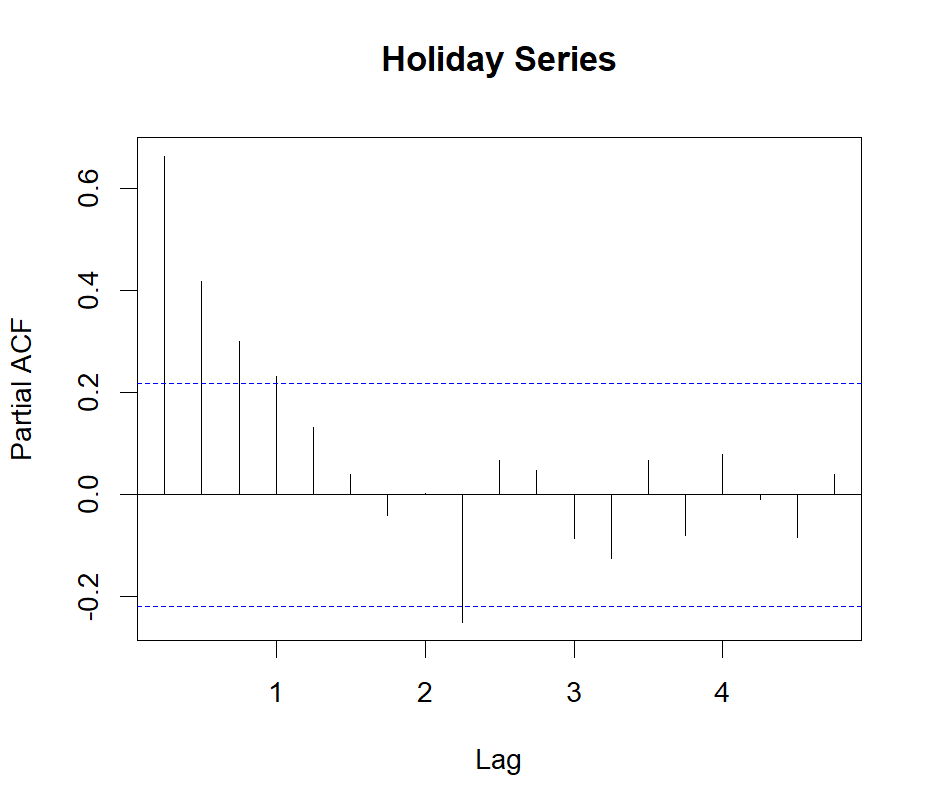
\includegraphics[width=0.65\linewidth]{fig/y2pacf.png}
\end{figure}

\noindent \noindent The PACF shows a large positive spike at lag 1, while most of the remaining partial autocorrelations are within the reference limits, except for a noticeable spike at lag 2. The PACF shows a large spike at lag 1, indicating that the first lag has a strong direct influence on the current observation. Most other lags are insignificant.

\noindent Taken together, the ACF and PACF indicate that the Holiday series is \textbf{non-stationary}, mainly due to the presence of a trend component. Therefore, differencing should be considered to remove the trend and achieve stationarity before fitting an ARIMA or SARIMA model.

